\documentclass[11pt]{article}

\usepackage[margin=1in]{geometry}
\usepackage[T1]{fontenc}
\usepackage[utf8]{inputenc}
\usepackage{lmodern}
\usepackage{microtype}
\usepackage{graphicx}
\usepackage{booktabs}
\usepackage{array}
\usepackage{longtable}
\usepackage{float}
\usepackage{caption}
\usepackage{subcaption}
\usepackage{xcolor}
\usepackage{hyperref}
\usepackage{url}
\usepackage{listings}

\graphicspath{{deliverables/final_assets/}{final_assets/}}
% Top-level final_assets PNGs use the neutral report theme (#F7F9FC)
% generated by scripts/render_final_charts.py and scripts/render_final_flowcharts.py.

\hypersetup{
  colorlinks=true,
  linkcolor=blue!50!black,
  urlcolor=blue!50!black,
  citecolor=blue!50!black
}

\lstset{
  basicstyle=\ttfamily\small,
  breaklines=true,
  frame=single,
  columns=fullflexible,
  backgroundcolor=\color{gray!6}
}

\title{\textbf{Ragebait Detection with Weak-Label Baselines and Gold-Label Supervision}}
\author{Group 8: Edison Cheah, Giuseppe Galiazzi, Lawson Herger, Andrew Lin\\
CS 4375.001 Machine Learning\\
\url{https://github.com/giuseppegaliazzitx-bit/ML-Project-Ragebait}}
\date{Spring 2026}

\begin{document}
\maketitle

\begin{abstract}
This project studies supervised detection of rage-inducing and abusive short social-media posts. The repository contains two research phases. Iteration 1 built a large weakly labeled binary pipeline over 507,682 posts using an instruction-tuned LLM; it was useful engineering scaffolding, but its scores measured agreement with model-generated labels rather than human judgment. Iteration 2 is the final benchmark: a 12,490-example human-labeled corpus with five classes, evaluated under both binary and multiclass formulations. The final CUDA complete-metrics artifacts show that fine-tuned \texttt{bert-base-uncased} is the strongest model on both tasks. On the held-out binary test split, BERT reaches 0.9055 accuracy, 0.9054 precision, 0.9395 recall, and 0.9222 F1. On the five-class test split, BERT reaches 0.7390 accuracy, 0.7390 micro F1, 0.6405 macro F1, and 0.7441 weighted F1. The main technical finding is not merely that BERT wins, but that the multiclass task exposes the remaining semantic difficulty: the model still confuses trolling, derogatory abuse, profanity, and hate speech when short posts combine insult, provocation, and target ambiguity.
\end{abstract}

\section{Introduction}

Ragebait is content designed to provoke anger, frustration, or outrage because those reactions drive replies, quote-posts, and downstream amplification. The machine-learning problem is difficult because ragebait is not identical to profanity, toxicity, or political disagreement. A post may be profane without being strategically provocative, and a post may be provocative without using obvious abusive vocabulary. The task therefore requires a model that can distinguish normal text from abusive or rage-inducing text, and, in the more difficult formulation, separate several overlapping abuse categories.

The project began with a high-volume weak-supervision approach. Iteration 1 unified multiple social-media sources, weak-labeled them with \texttt{Qwen/Qwen2.5-3B-Instruct-AWQ}, and trained classical and BERT classifiers on a balanced high-confidence subset. The best archived weak-label BERT model achieved 0.8767 accuracy and 0.8735 macro F1. However, that result did not establish agreement with human labels; it established agreement with another model's labels. This motivated the final Iteration 2 design: use a smaller but human-labeled dataset, freeze one train/validation/test split, and compare a ladder of models under both binary and multiclass task definitions.

The final experiments use four model families. Tier 1 contains TF-IDF Logistic Regression and TF-IDF Linear SVC. Tier 2 is a PyTorch feed-forward neural network (FFNN) over train-only token embeddings with mean pooling. Tier 3 fine-tunes \texttt{bert-base-uncased}. The completed CUDA metrics artifacts under \path{deliverables/final_assets/complete_metrics/} are the authoritative source for all final numbers in this report.

\section{Data}

\subsection{Iteration 1 Weak-Label Corpus}

The archived weak-label track unified eight raw sources into a common schema with \texttt{post\_id}, \texttt{author\_id}, \texttt{created\_at}, \texttt{language}, \texttt{text}, and \texttt{source}. The import manifest records 507,682 rows after removing 31,439 duplicates. Weak labeling then produced 31,072 positive examples, or 6.12\% of the corpus. A high-confidence pool at confidence at least 0.95 contained 102,104 rows with a 12.68\% positive rate. The final archived training file, \path{data/labeled/balanced_32000_c95_r60_40.csv}, contained 32,000 rows with a 60/40 negative/positive class ratio.

The Iteration 1 corpus remains useful historically because it demonstrates data ingestion, weak labeling, balancing, and baseline training. It is not the final scientific benchmark because its labels are model-generated.

\subsection{Iteration 2 Gold-Label Corpus}

The final experiments use \path{iteration2/data/raw/trolldata.csv}, a 12,490-row human-labeled abusive-language dataset associated with the ``Trawling for Trolling'' dataset reference. The label distribution is shown in Table~\ref{tab:label-dist}.

\begin{table}[H]
\centering
\caption{Human-labeled Iteration 2 label distribution.}
\label{tab:label-dist}
\begin{tabular}{lrr}
\toprule
Label & Rows & Share \\
\midrule
Normal & 5,053 & 40.46\% \\
Profanity & 1,582 & 12.67\% \\
Trolling & 4,537 & 36.33\% \\
Derogatory & 862 & 6.90\% \\
Hate Speech & 456 & 3.65\% \\
\bottomrule
\end{tabular}
\end{table}

Two task framings are derived from these labels. The binary task maps \texttt{Normal} to 0 and all non-\texttt{Normal} labels to 1. The multiclass task preserves the five labels in this order: Normal, Profanity, Trolling, Derogatory, and Hate Speech. The binary framing answers whether a post should be flagged as normal versus abusive or rage-inducing. The multiclass framing asks which type of behavior is present, making it more diagnostically useful but substantially harder.

\subsection{Canonical Splits}

All final models use the same stratified 80/10/10 split with seed 42. The split is frozen in \path{iteration2/data/processed/} and summarized in Table~\ref{tab:splits}. Validation data is used for model selection or checkpoint selection; held-out test data is used for final claims.

\begin{table}[H]
\centering
\caption{Frozen Iteration 2 split sizes and binary class distribution.}
\label{tab:splits}
\begin{tabular}{lrrr}
\toprule
Split & Rows & Normal & Abusive/Ragebait \\
\midrule
Train & 9,992 & 4,042 & 5,950 \\
Validation & 1,249 & 506 & 743 \\
Test & 1,249 & 505 & 744 \\
\bottomrule
\end{tabular}
\end{table}

\begin{table}[H]
\centering
\caption{Frozen multiclass split distribution.}
\label{tab:multi-splits}
\begin{tabular}{lrrrrr}
\toprule
Split & Normal & Profanity & Trolling & Derogatory & Hate Speech \\
\midrule
Train & 4,042 & 1,265 & 3,630 & 690 & 365 \\
Validation & 506 & 158 & 454 & 86 & 45 \\
Test & 505 & 159 & 453 & 86 & 46 \\
\bottomrule
\end{tabular}
\end{table}

\section{Methodology}

\subsection{Preprocessing and Feature Construction}

The Iteration 2 dataset builder validates required columns, strips empty text and label fields, assigns stable row IDs, maps labels, and writes split manifests. Text cleaning is intentionally conservative in the final benchmark: no aggressive deletion of punctuation, profanity, or user-facing lexical cues is applied before TF-IDF or BERT. This is appropriate because profanity, punctuation, casing patterns, and slang can carry signal for abuse detection.

Tier 1 models use scikit-learn TF-IDF features with 20,000 maximum features, unigram and bigram features, \texttt{min\_df = 2}, \texttt{max\_df = 0.95}, and sublinear term frequency. Tier 2 builds a train-only vocabulary with lowercasing, a minimum frequency of 2, maximum vocabulary size 20,000, and maximum sequence length 64. The final vocabulary size in the complete metrics run is 10,975. Tier 3 uses the \texttt{bert-base-uncased} WordPiece tokenizer with maximum length 128 for both final binary and multiclass BERT runs.

\subsection{Class Imbalance}

The binary task is not perfectly balanced but is close enough that no synthetic balancing is used in Iteration 2. The multiclass task is highly imbalanced, especially for Hate Speech and Derogatory. Multiclass training therefore uses inverse-frequency class weights computed from the train split:

\[
w_i = \frac{N}{K \cdot n_i}
\]

where \(N\) is the number of training examples, \(K\) is the number of classes, and \(n_i\) is the training count for class \(i\). The resulting weights are Normal 0.4944, Profanity 1.5798, Trolling 0.5505, Derogatory 2.8962, and Hate Speech 5.4751. These weights are used by the multiclass FFNN and multiclass BERT losses.

\subsection{Model Families}

\paragraph{Logistic Regression.}
Logistic Regression is a linear classifier over TF-IDF features. It estimates a separating hyperplane while producing calibrated-style decision scores through the logistic link. In this project it is a strong lexical baseline because many abusive examples contain recurring words, insults, and bigrams. The binary configuration uses the \texttt{liblinear} solver; the multiclass configuration uses the scikit-learn Logistic Regression implementation with a larger iteration limit and class weights.

\paragraph{Linear SVC.}
Linear SVC is a maximum-margin linear classifier over the same TF-IDF representation. It is often competitive on sparse text because a linear decision boundary over many lexical features can separate strong n-gram cues efficiently. In this project it is the fastest and strongest non-transformer on the final binary test F1, but it lacks contextual representation and therefore struggles with subtle multiclass distinctions.

\paragraph{Feed-forward Neural Network.}
The FFNN learns token embeddings from the training split, masks padding, mean-pools token embeddings, and applies hidden layers with ReLU and dropout. Listing~\ref{lst:ffnn} shows the central representation step. This model can learn nonlinear interactions, but mean pooling discards word order and pragmatic structure. Its results confirm that a shallow neural network is not automatically better than a strong linear text baseline.

\begin{lstlisting}[language=Python, caption={Mean-pooled FFNN representation used by Tier 2.}, label={lst:ffnn}]
embeddings = self.embedding(input_ids)
mask = (input_ids != self.pad_index).unsqueeze(-1)
masked_embeddings = embeddings * mask
pooled_embeddings = masked_embeddings.sum(dim=1) / mask.sum(dim=1).clamp(min=1)
logits = self.classifier(pooled_embeddings)
\end{lstlisting}

\paragraph{BERT Sequence Classifier.}
BERT uses contextual bidirectional transformer representations. The implementation loads \texttt{bert-base-uncased}, applies dropout to the pooled encoder output, and uses a linear classifier head. Training uses AdamW, weight-decay parameter groups, linear warmup/decay scheduling, gradient clipping, dynamic padding, and CUDA automatic mixed precision when available. The final binary BERT run trains for three epochs and selects epoch 2 by validation F1. The final multiclass BERT run trains for four epochs and selects epoch 4 by validation macro F1.

\paragraph{Legacy Models.}
The archived Iteration 1 code also tested Gaussian Naive Bayes and Decision Tree classifiers. Those models are not in the final Iteration 2 complete metrics artifact, so they are not used for final benchmark claims. In the archived tuned weak-label baseline run, raw-text Gaussian NB reached 0.6427 accuracy and raw-text Decision Tree reached 0.6729 accuracy, both far below raw-text Linear SVC at 0.8744 accuracy.

\section{Implementation}

The active implementation lives under \path{iteration2/}. Data preparation is handled by \path{iteration2/src/data/make_dataset.py}; feature construction and class weighting are handled by \path{iteration2/src/data/preprocessing.py}; model definitions are in \path{iteration2/src/models/}; and evaluation utilities are in \path{iteration2/src/evaluation/}. The final complete metrics were generated by \path{scripts/compute_complete_final_metrics.py}, which writes artifacts into \path{deliverables/final_assets/complete_metrics/}.

The final artifact package includes JSON summaries, training histories, tokenizer snapshots, prediction CSVs for binary BERT, hard-error CSVs for multiclass BERT, and confusion matrices. This matters because the final report can audit the model outputs without relying on old slide drafts or manually copied tables.

\begin{figure}[H]
\centering
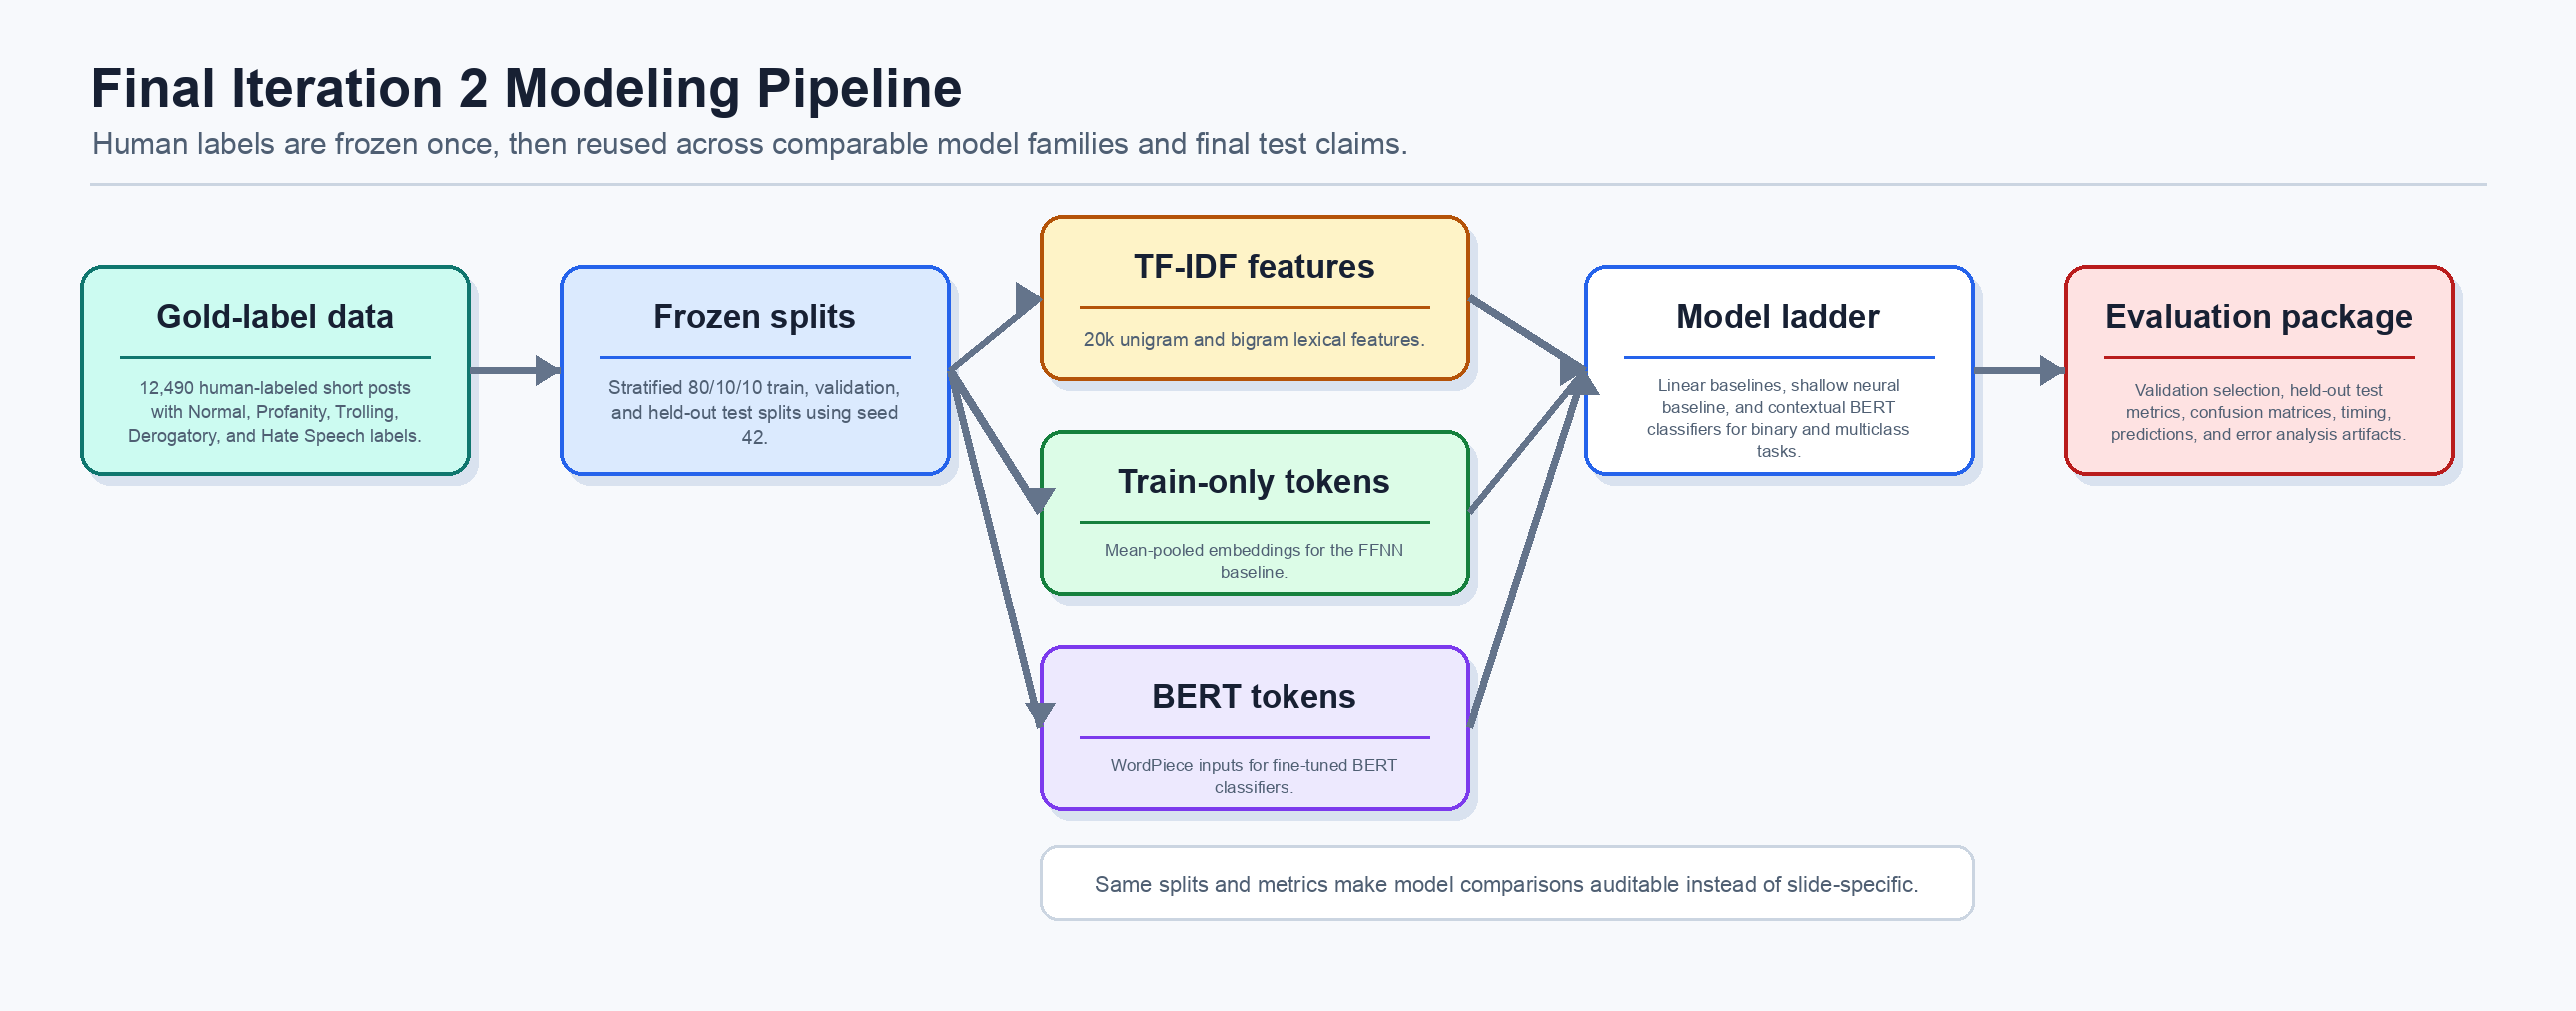
\includegraphics[width=\linewidth]{pipeline_flowchart.png}
\caption{Final Iteration 2 pipeline from human-labeled data through split freezing, representation, model training, and evaluation.}
\label{fig:pipeline}
\end{figure}

\section{Experiments and Results}

\subsection{Evaluation Metrics}

Binary classification reports accuracy, precision, recall, and F1 for the positive class. Precision measures how often predicted ragebait or abusive posts are correct; recall measures how much of the true abusive class is recovered; F1 balances those two. Multiclass classification reports accuracy, micro F1, macro precision, macro recall, macro F1, weighted F1, and per-class precision/recall/F1. Macro F1 is especially important because it gives equal weight to rare classes such as Hate Speech rather than allowing majority classes to dominate the score.

\subsection{Validation Results and Model Selection}

The validation split is used to compare models during development and to select neural checkpoints. Table~\ref{tab:binary-val} shows the binary validation metrics. BERT has the best validation F1 at 0.9302, and the selected complete-metrics checkpoint is epoch 2.

\begin{table}[H]
\centering
\caption{Binary validation results from the complete metrics artifact.}
\label{tab:binary-val}
\begin{tabular}{lrrrr}
\toprule
Model & Accuracy & Precision & Recall & F1 \\
\midrule
Logistic Regression & 0.8695 & 0.8545 & 0.9408 & 0.8956 \\
Linear SVC & 0.8831 & 0.8912 & 0.9152 & 0.9031 \\
FFNN & 0.8903 & 0.8966 & 0.9219 & 0.9091 \\
BERT & \textbf{0.9159} & \textbf{0.9186} & \textbf{0.9421} & \textbf{0.9302} \\
\bottomrule
\end{tabular}
\end{table}

Table~\ref{tab:multi-val} shows the multiclass validation metrics. BERT again leads, with 0.6828 validation macro F1. The multiclass BERT checkpoint is epoch 4, selected by validation macro F1.

\begin{table}[H]
\centering
\caption{Multiclass validation results from the complete metrics artifact.}
\label{tab:multi-val}
\begin{tabular}{lrrrr}
\toprule
Model & Accuracy & Micro F1 & Macro F1 & Weighted F1 \\
\midrule
Logistic Regression & 0.6869 & 0.6869 & 0.6044 & 0.6933 \\
Linear SVC & 0.7038 & 0.7038 & 0.6027 & 0.7030 \\
FFNN & 0.6934 & 0.6934 & 0.5969 & 0.7009 \\
BERT & \textbf{0.7526} & \textbf{0.7526} & \textbf{0.6828} & \textbf{0.7589} \\
\bottomrule
\end{tabular}
\end{table}

\subsection{Binary Classification}

Table~\ref{tab:binary-test} reports the final held-out binary test results from \path{complete_metrics.json}. BERT is best, but the margin should be interpreted against strong baselines rather than weak strawmen. The best non-transformer F1 is Linear SVC at 0.8884; BERT reaches 0.9222, a gain of 0.0337 F1. BERT also has the highest recall at 0.9395 while preserving precision above 0.905.

\begin{table}[H]
\centering
\caption{Binary held-out test results.}
\label{tab:binary-test}
\begin{tabular}{lrrrr}
\toprule
Model & Accuracy & Precision & Recall & F1 \\
\midrule
Logistic Regression & 0.8551 & 0.8371 & 0.9395 & 0.8854 \\
Linear SVC & 0.8655 & 0.8780 & 0.8992 & 0.8884 \\
FFNN & 0.8655 & 0.8789 & 0.8978 & 0.8883 \\
BERT & \textbf{0.9055} & \textbf{0.9054} & \textbf{0.9395} & \textbf{0.9222} \\
\bottomrule
\end{tabular}
\end{table}

\begin{figure}[H]
\centering
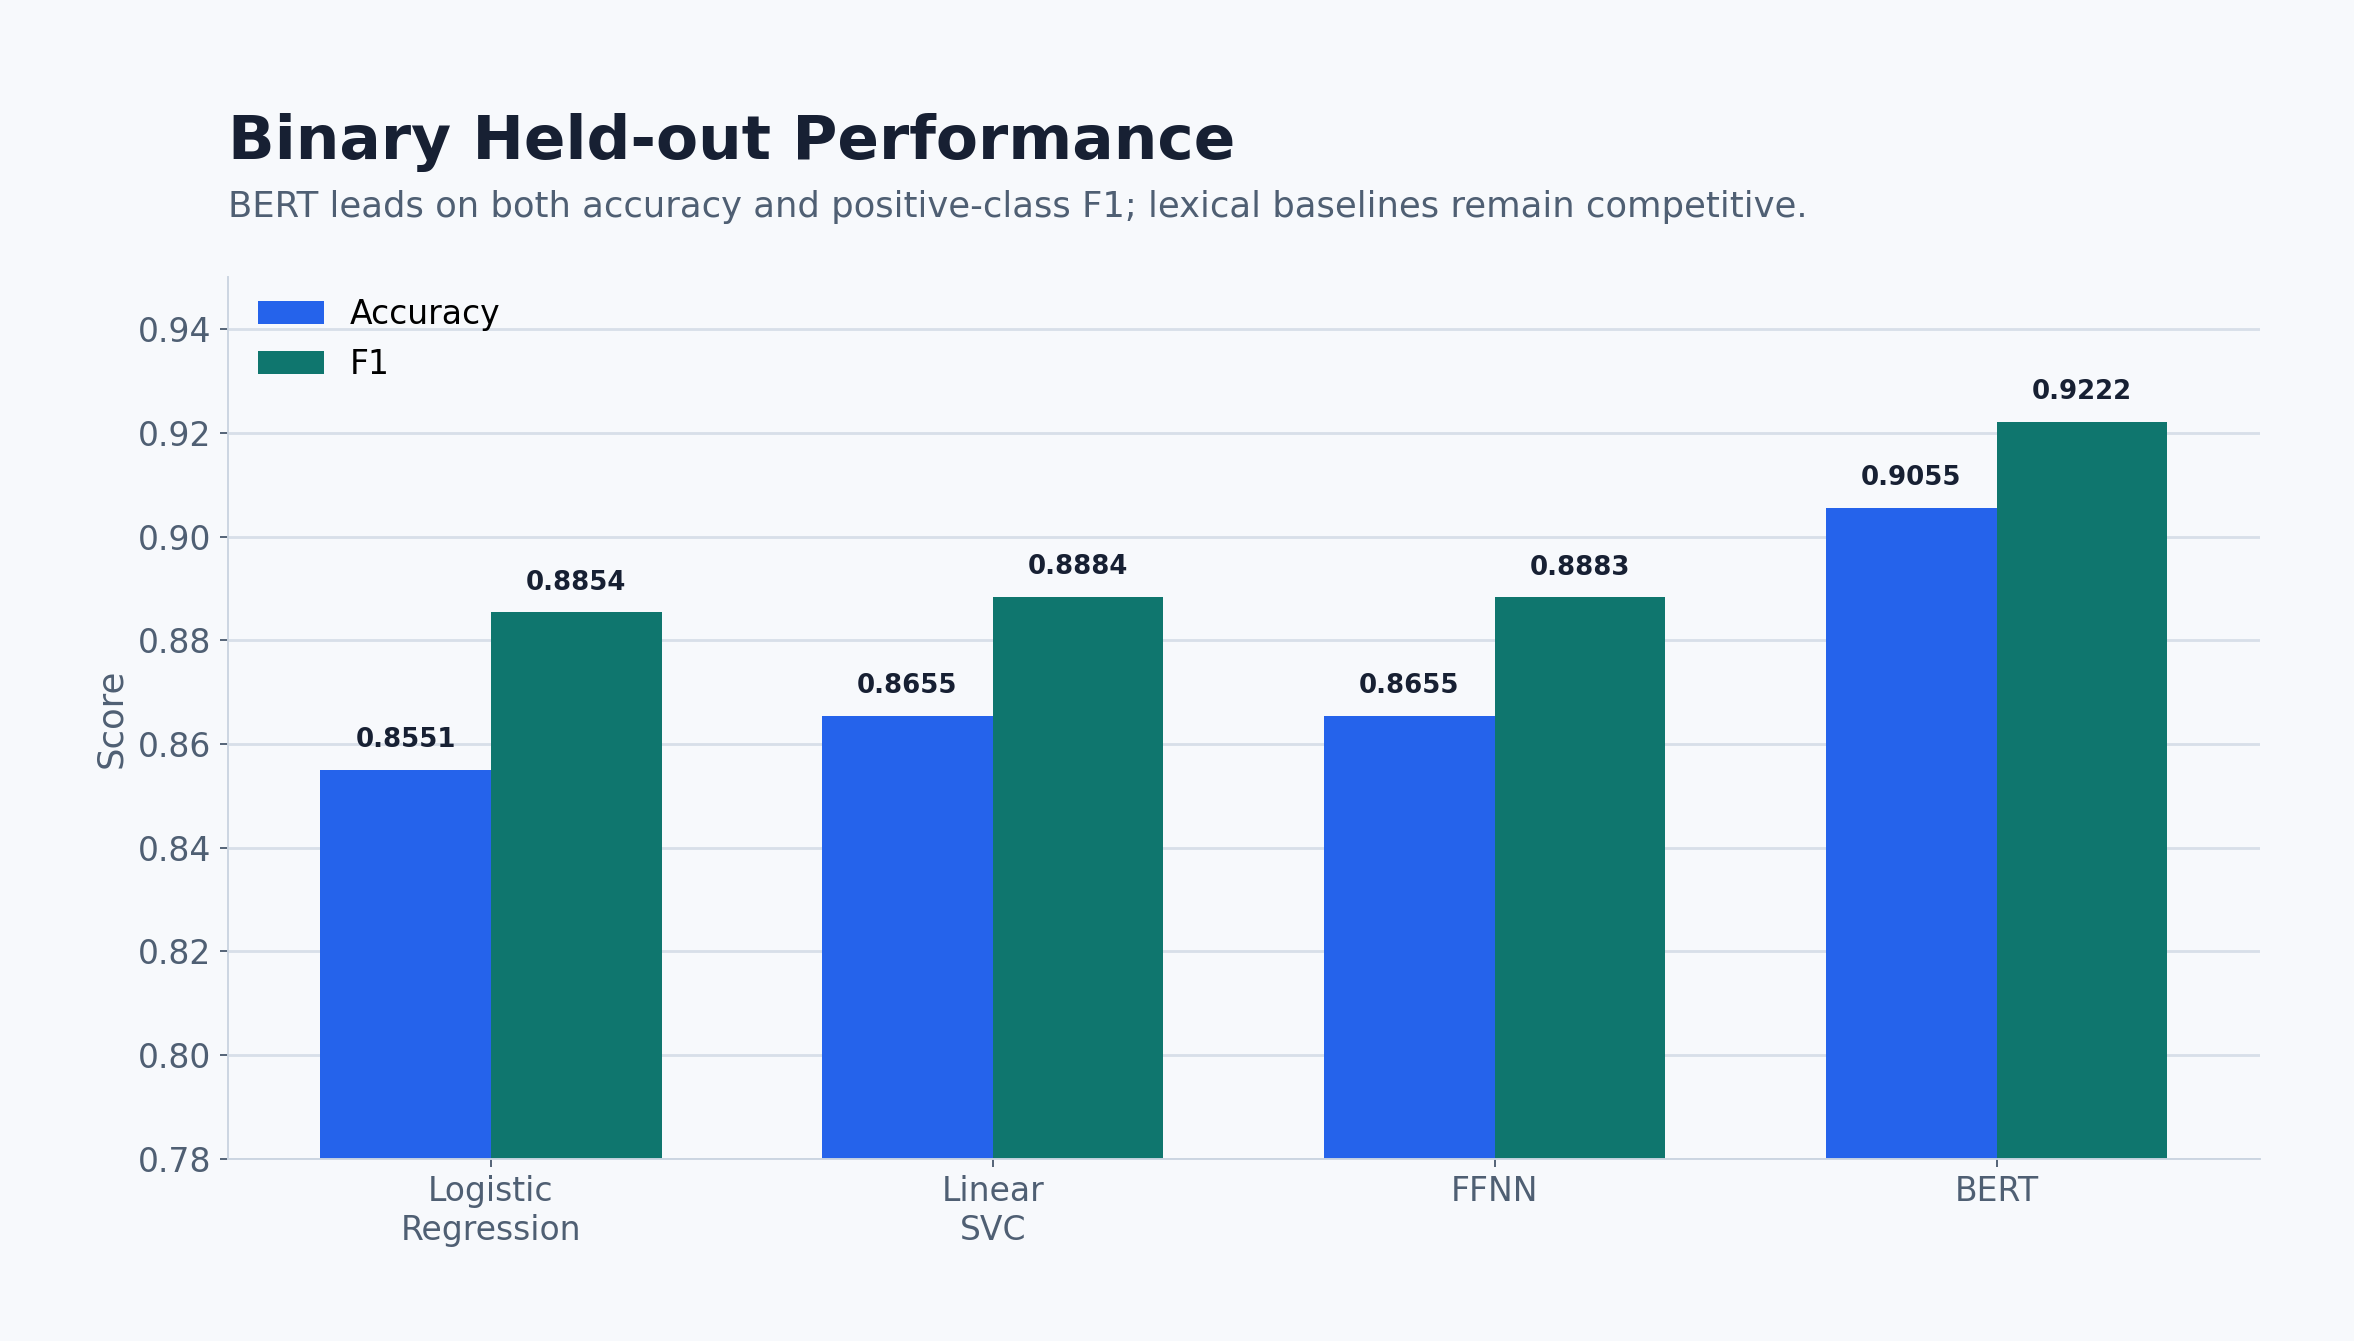
\includegraphics[width=.94\linewidth]{binary_model_comparison.png}
\caption{Binary held-out accuracy and F1. BERT improves over all non-transformer models, but TF-IDF baselines remain strong.}
\label{fig:binary-bars}
\end{figure}

The BERT binary confusion matrix is shown in Table~\ref{tab:binary-cm}. The model correctly identifies 699 of 744 abusive/ragebait examples and 432 of 505 normal examples. The main operational tradeoff is 73 false positives against 45 false negatives: the model is tuned toward recovering abusive posts, which is reflected in its higher recall than precision.

\begin{table}[H]
\centering
\caption{Binary BERT held-out test confusion matrix from saved test predictions.}
\label{tab:binary-cm}
\begin{tabular}{lrr}
\toprule
 & Predicted Normal & Predicted Ragebait/Abusive \\
\midrule
True Normal & 432 & 73 \\
True Ragebait/Abusive & 45 & 699 \\
\bottomrule
\end{tabular}
\end{table}

\subsection{Multiclass Classification}

Table~\ref{tab:multi-test} reports the final five-class test results. The multiclass setting is substantially harder because the model must distinguish normal language, general profanity, trolling, derogatory abuse, and hate speech. BERT reaches 0.6405 macro F1, compared with 0.5524 for the best non-transformer baseline, a gain of 0.0881. The larger gain on multiclass than binary classification is the strongest evidence that contextual representation matters most when the label boundary depends on target and intent.

\begin{table}[H]
\centering
\caption{Multiclass held-out test results.}
\label{tab:multi-test}
\begin{tabular}{lrrrr}
\toprule
Model & Accuracy & Micro F1 & Macro F1 & Weighted F1 \\
\midrule
Logistic Regression & 0.6645 & 0.6645 & 0.5524 & 0.6718 \\
Linear SVC & 0.6797 & 0.6797 & 0.5403 & 0.6764 \\
FFNN & 0.6517 & 0.6517 & 0.5250 & 0.6606 \\
BERT & \textbf{0.7390} & \textbf{0.7390} & \textbf{0.6405} & \textbf{0.7441} \\
\bottomrule
\end{tabular}
\end{table}

\begin{figure}[H]
\centering
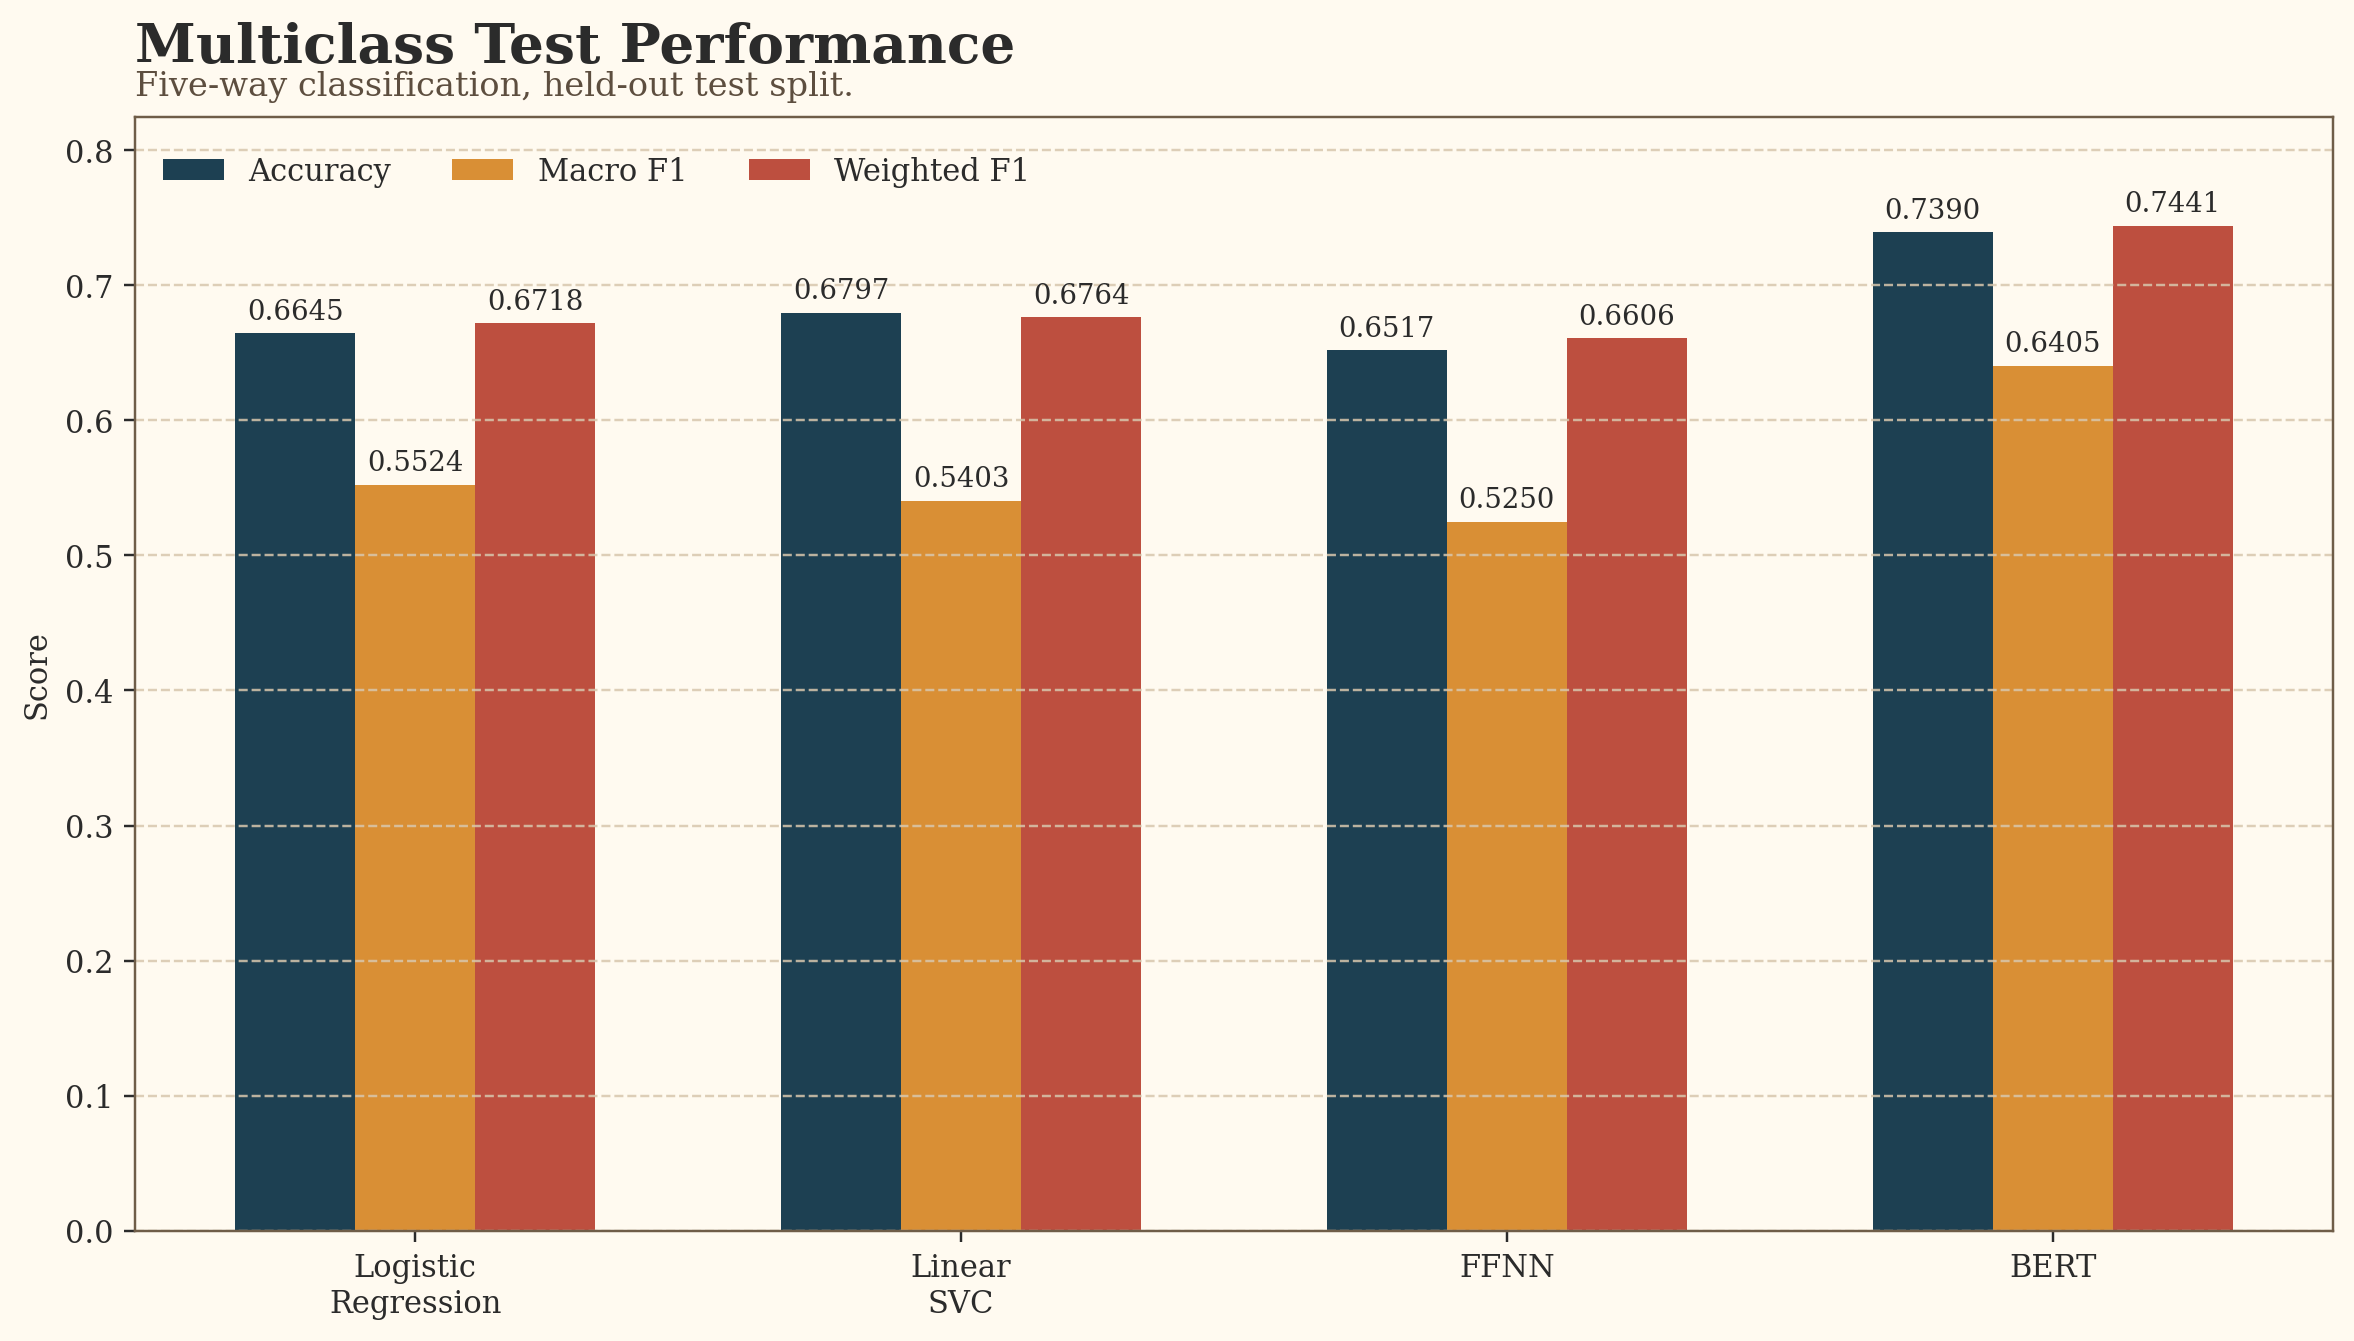
\includegraphics[width=.94\linewidth]{multiclass_model_comparison.png}
\caption{Five-class held-out metrics. Macro F1 exposes the difficulty of minority abusive categories.}
\label{fig:multi-bars}
\end{figure}

\subsection{Class-wise Results}

Table~\ref{tab:classwise} compares the strongest non-transformer multiclass model, Logistic Regression, against BERT. BERT improves every class. Profanity improves from 0.6108 F1 to 0.7349 F1; Derogatory improves from 0.3398 to 0.4384; Hate Speech improves from 0.3696 to 0.4667. These gains are meaningful, but the tail classes remain the hardest categories.

\begin{table}[H]
\centering
\caption{Class-wise held-out F1: Logistic Regression versus BERT.}
\label{tab:classwise}
\begin{tabular}{lrrr}
\toprule
Class & Logistic Regression F1 & BERT F1 & Gain \\
\midrule
Normal & 0.8215 & 0.8772 & 0.0557 \\
Profanity & 0.6108 & 0.7349 & 0.1241 \\
Trolling & 0.6202 & 0.6853 & 0.0651 \\
Derogatory & 0.3398 & 0.4384 & 0.0986 \\
Hate Speech & 0.3696 & 0.4667 & 0.0971 \\
\bottomrule
\end{tabular}
\end{table}

\begin{figure}[H]
\centering
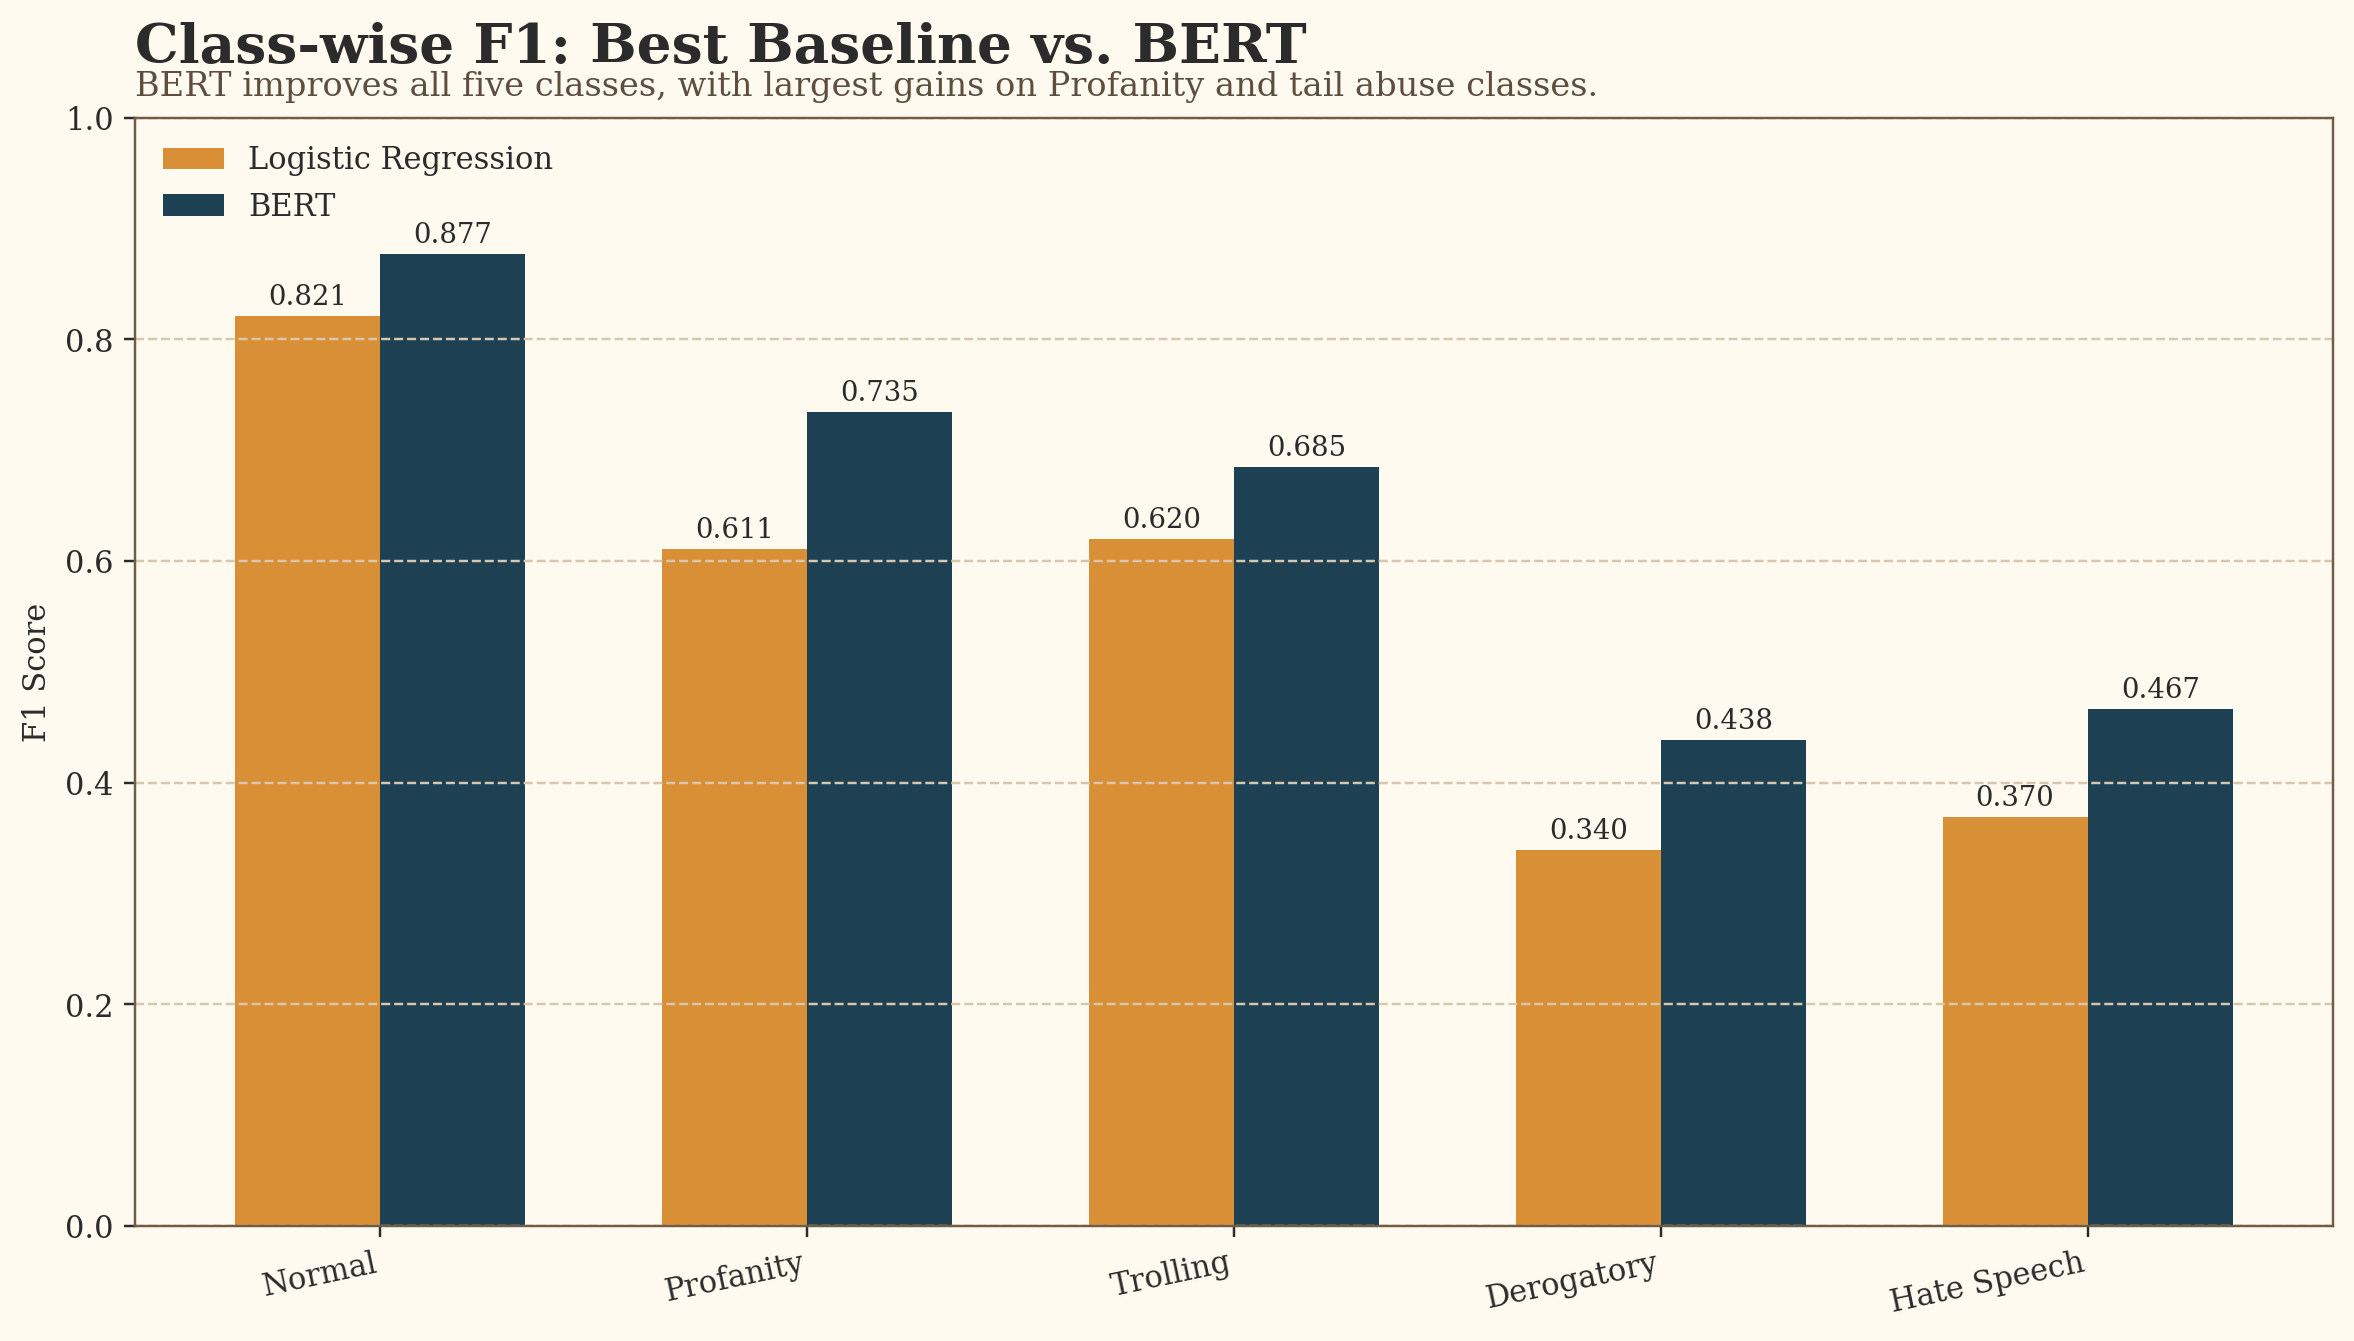
\includegraphics[width=.94\linewidth]{classwise_f1_comparison.png}
\caption{Class-wise F1 for Logistic Regression and BERT. The largest absolute gain is on Profanity, while Derogatory and Hate Speech remain difficult.}
\label{fig:classwise-bars}
\end{figure}

\subsection{Binary Versus Multiclass Framing}

The binary task and multiclass task answer different questions. Binary classification is useful for coarse screening: should this post be treated as normal or as rage-inducing/abusive? It produces high F1 because obvious lexical signals are often enough. Multiclass classification is useful for diagnosis and intervention: is the post merely profane, intentionally trolling, derogatory, or hateful? It is harder because one short post can contain several signals at once.

\begin{figure}[H]
\centering
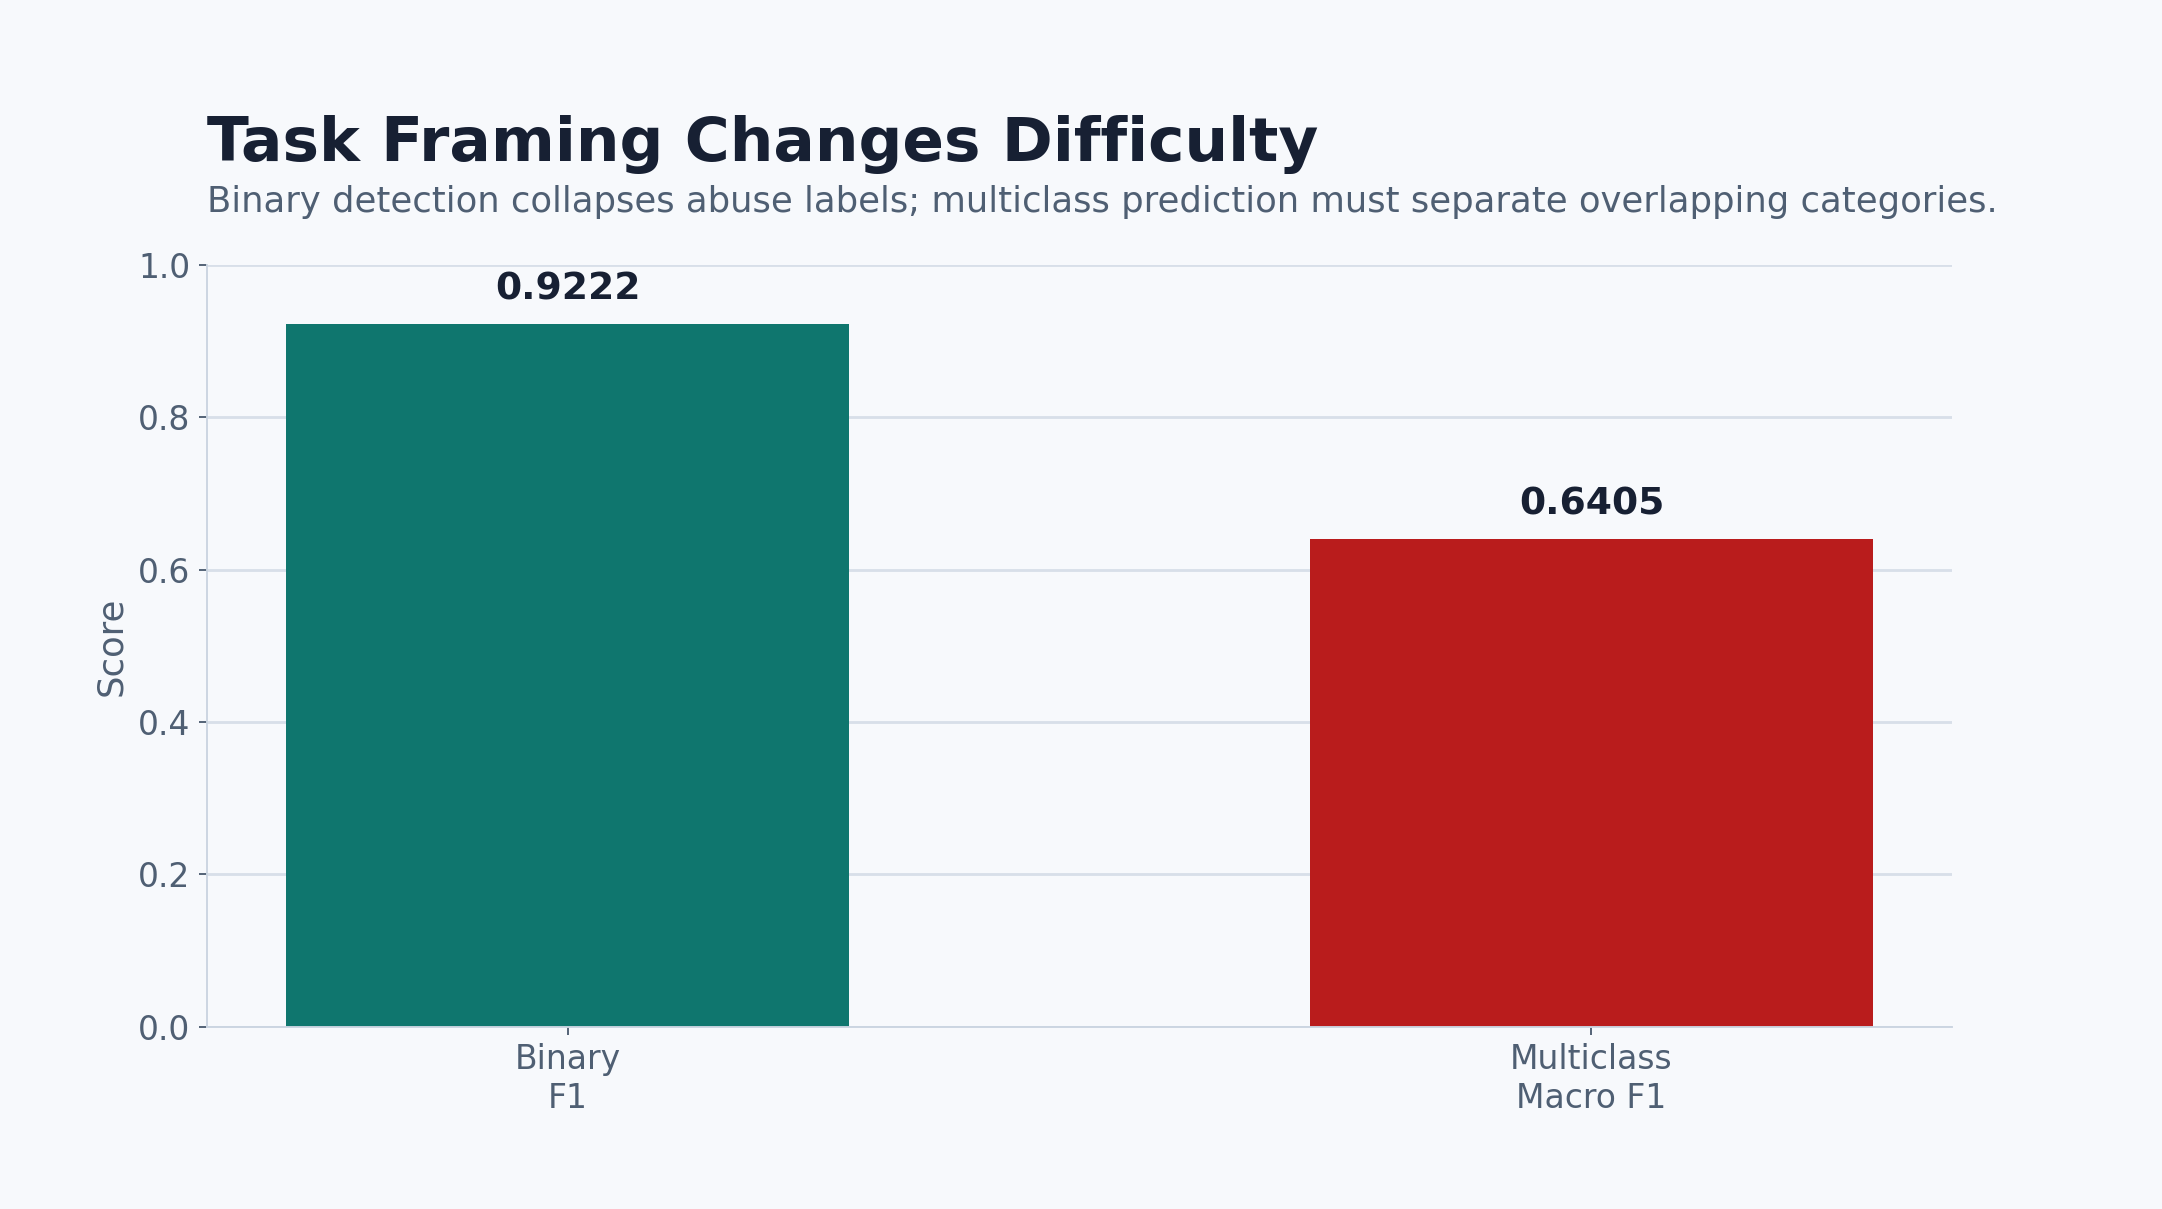
\includegraphics[width=.82\linewidth]{binary_vs_multiclass_bert.png}
\caption{BERT performance by task framing. The binary task reaches 0.9222 F1; the five-class task reaches 0.6405 macro F1.}
\label{fig:framing}
\end{figure}

\begin{figure}[H]
\centering
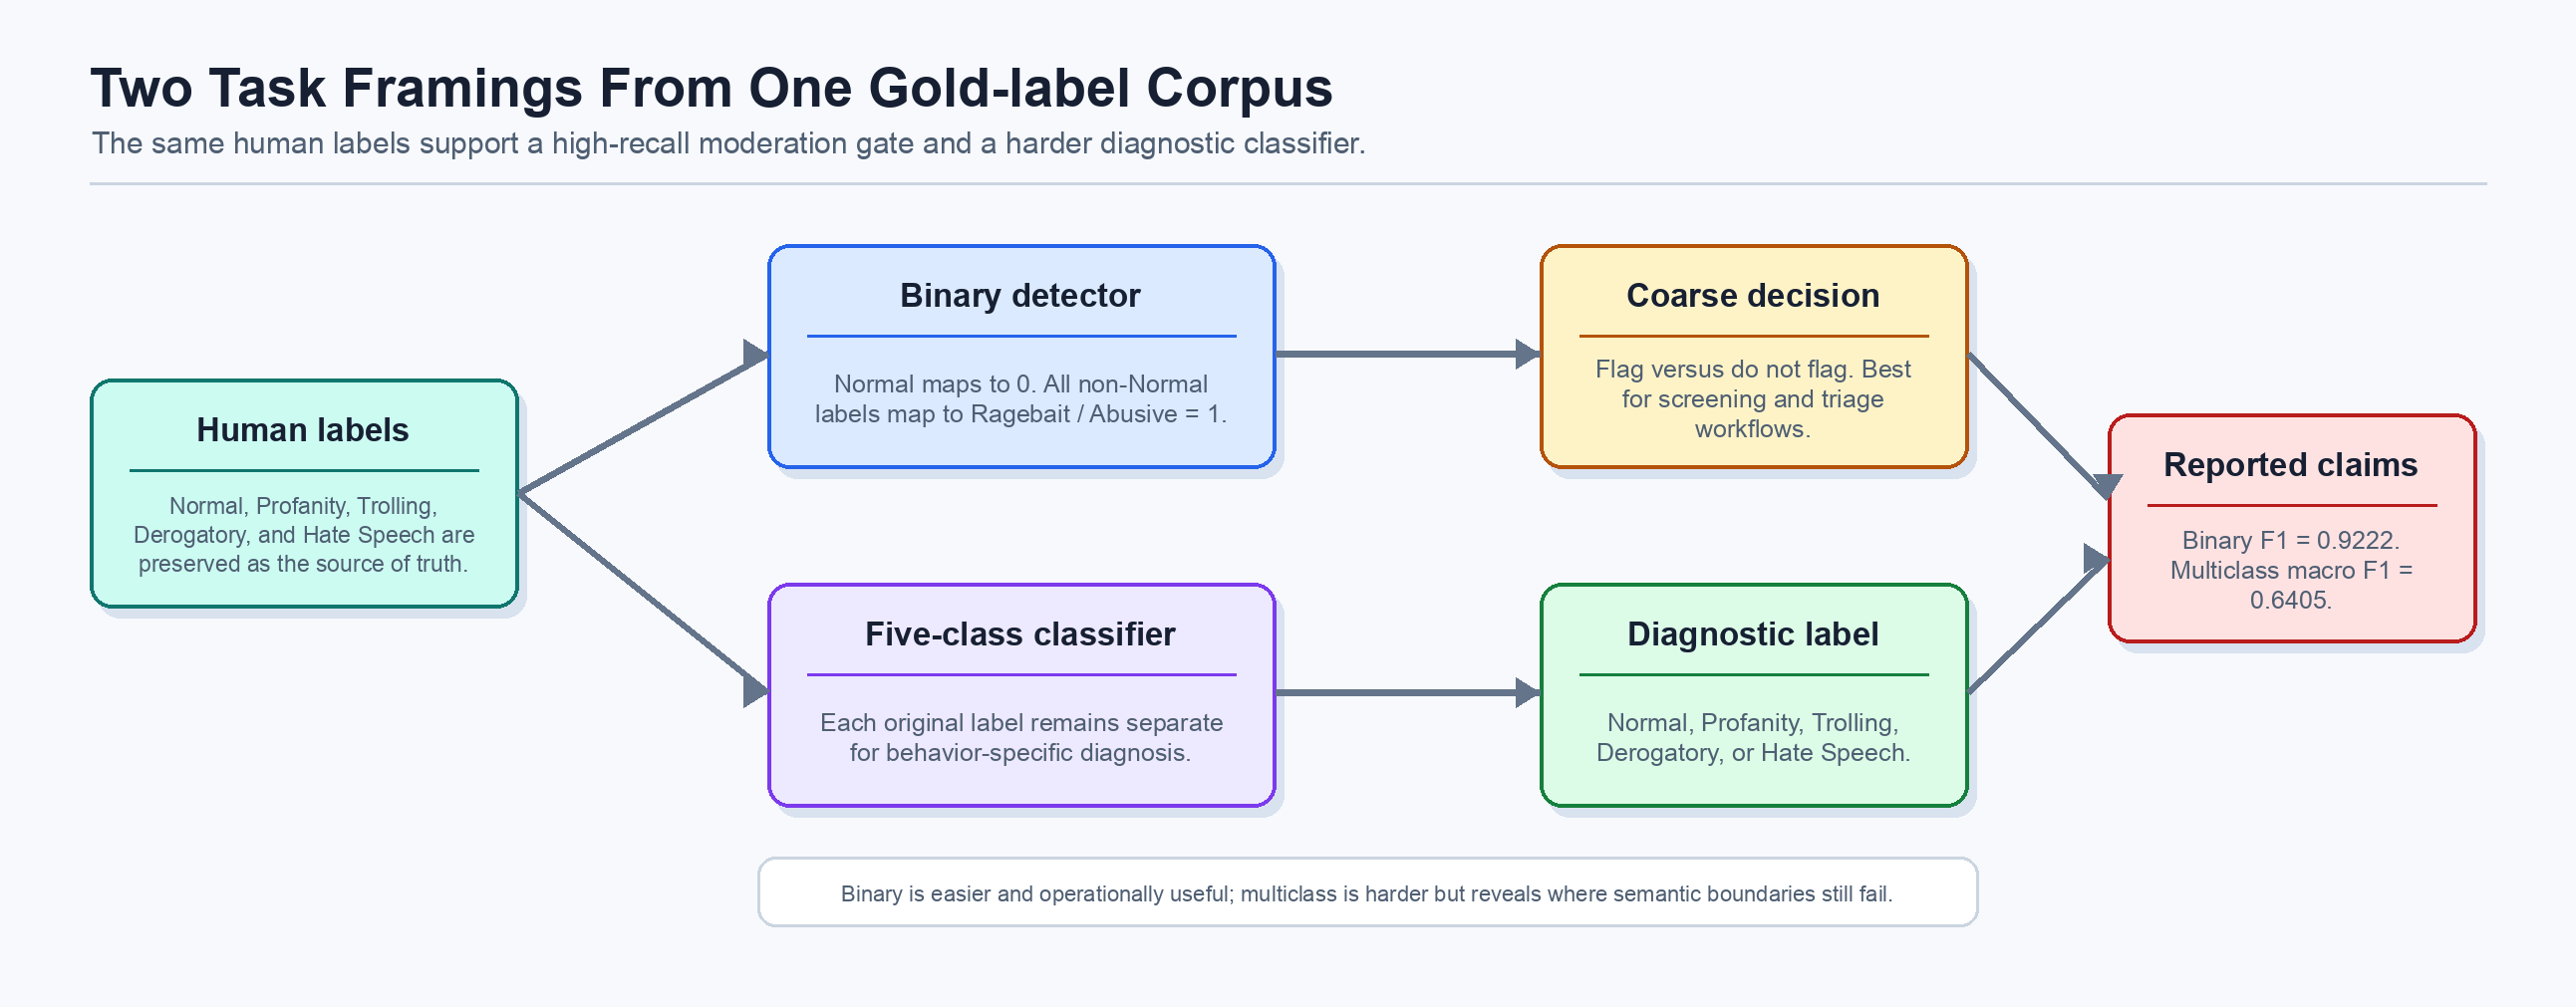
\includegraphics[width=\linewidth]{task_framing_flowchart.png}
\caption{The same gold labels support a coarse binary detector and a more diagnostic five-class classifier.}
\label{fig:task-flow}
\end{figure}

\subsection{Error Analysis}

The multiclass BERT confusion matrix artifact and class-wise metrics show that errors are not evenly distributed. Normal has strong F1 at 0.8772, and Profanity has strong recall at 0.8805. The weaker classes are Derogatory and Hate Speech, with F1 scores of 0.4384 and 0.4667. Trolling is also a boundary class: its recall is 0.6225, meaning many true trolling examples are assigned to neighboring categories.

\begin{figure}[H]
\centering
\begin{subfigure}{.48\linewidth}
\centering
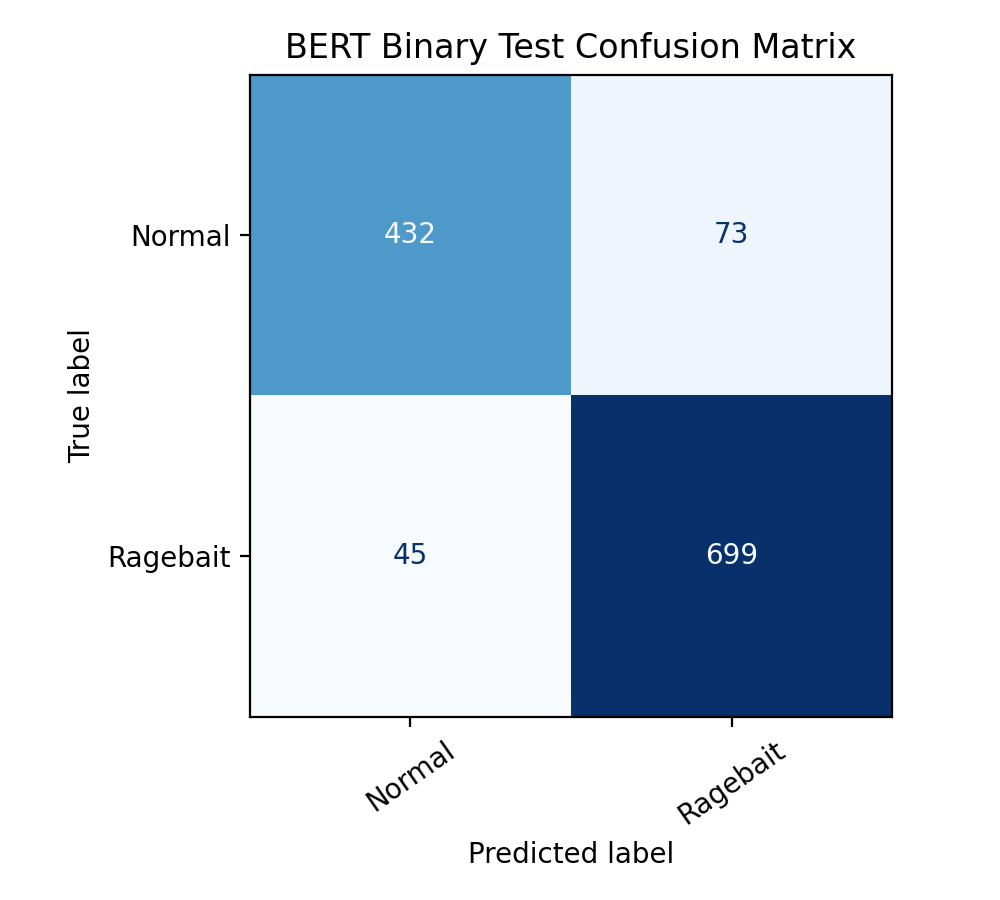
\includegraphics[width=\linewidth]{complete_metrics/binary_bert/bert_test_confusion_matrix.png}
\caption{Binary BERT test confusion matrix.}
\end{subfigure}
\hfill
\begin{subfigure}{.48\linewidth}
\centering

\includegraphics[width=\linewidth]{complete_metrics/multiclass_bert/bert_test_confusion_matrix.png}
\caption{Multiclass BERT test confusion matrix.}
\end{subfigure}
\caption{Confusion matrix artifacts generated by the complete metrics run.}
\label{fig:cms}
\end{figure}

The saved hard-error file for multiclass BERT contains 95 targeted high-confidence mistakes from two confusion families. It includes 68 \texttt{Trolling} examples predicted as \texttt{Derogatory}, 25 \texttt{Derogatory} examples predicted as \texttt{Trolling}, and 2 \texttt{Hate Speech} examples predicted as \texttt{Profanity}. The highest-confidence miss is a Hate Speech example predicted as Profanity with confidence 0.9632; the content includes explicit profanity, but the gold label reflects a wish of harm. Other high-confidence errors are insult-heavy posts labeled Trolling by humans but predicted as Derogatory by the model. These examples show that the remaining failures are semantic boundary failures, not merely missing vocabulary.

To check the unknown-word explanation, the train-only FFNN vocabulary was rebuilt from the multiclass train split. The overall multiclass test token OOV rate is 7.83\%, and the targeted hard-error OOV rate is 7.61\%. The mean per-document OOV rate is 8.56\% for the full test set and 8.74\% for the targeted hard-error subset. Because the hard-error subset does not have a dramatically higher OOV rate, the main issue is label-boundary semantics rather than unseen tokens alone.

\subsection{Compute and Speed Analysis}

Table~\ref{tab:timing} reports the final timing fields from \path{complete_metrics.json}. Classical TF-IDF models are effectively free to train and evaluate. FFNN training remains cheap. BERT is much more expensive, but the CUDA complete-metrics run makes the cost practical for offline or batch evaluation. Binary BERT trains in 173.2670 seconds and evaluates the test split in 3.4112 seconds. Multiclass BERT trains in 279.6823 seconds; its saved prediction timing is 7.5751 seconds for the validation plus test evaluation pass used by the trainer.

\begin{table}[H]
\centering
\caption{Timing from the complete metrics artifact.}
\label{tab:timing}
\begin{tabular}{llrr}
\toprule
Task & Model & Train seconds & Evaluation / predict seconds \\
\midrule
Binary & Logistic Regression & 0.0362 & 0.0002 \\
Binary & Linear SVC & 0.0296 & 0.0001 \\
Binary & FFNN & 13.6128 & 0.0395 \\
Binary & BERT & 173.2670 & 3.4112 \\
Multiclass & Logistic Regression & 7.4438 & 0.0006 \\
Multiclass & Linear SVC & 0.1864 & 0.0003 \\
Multiclass & FFNN & 23.6989 & 0.0465 \\
Multiclass & BERT & 279.6823 & 7.5751 \\
\bottomrule
\end{tabular}
\end{table}

\begin{figure}[H]
\centering
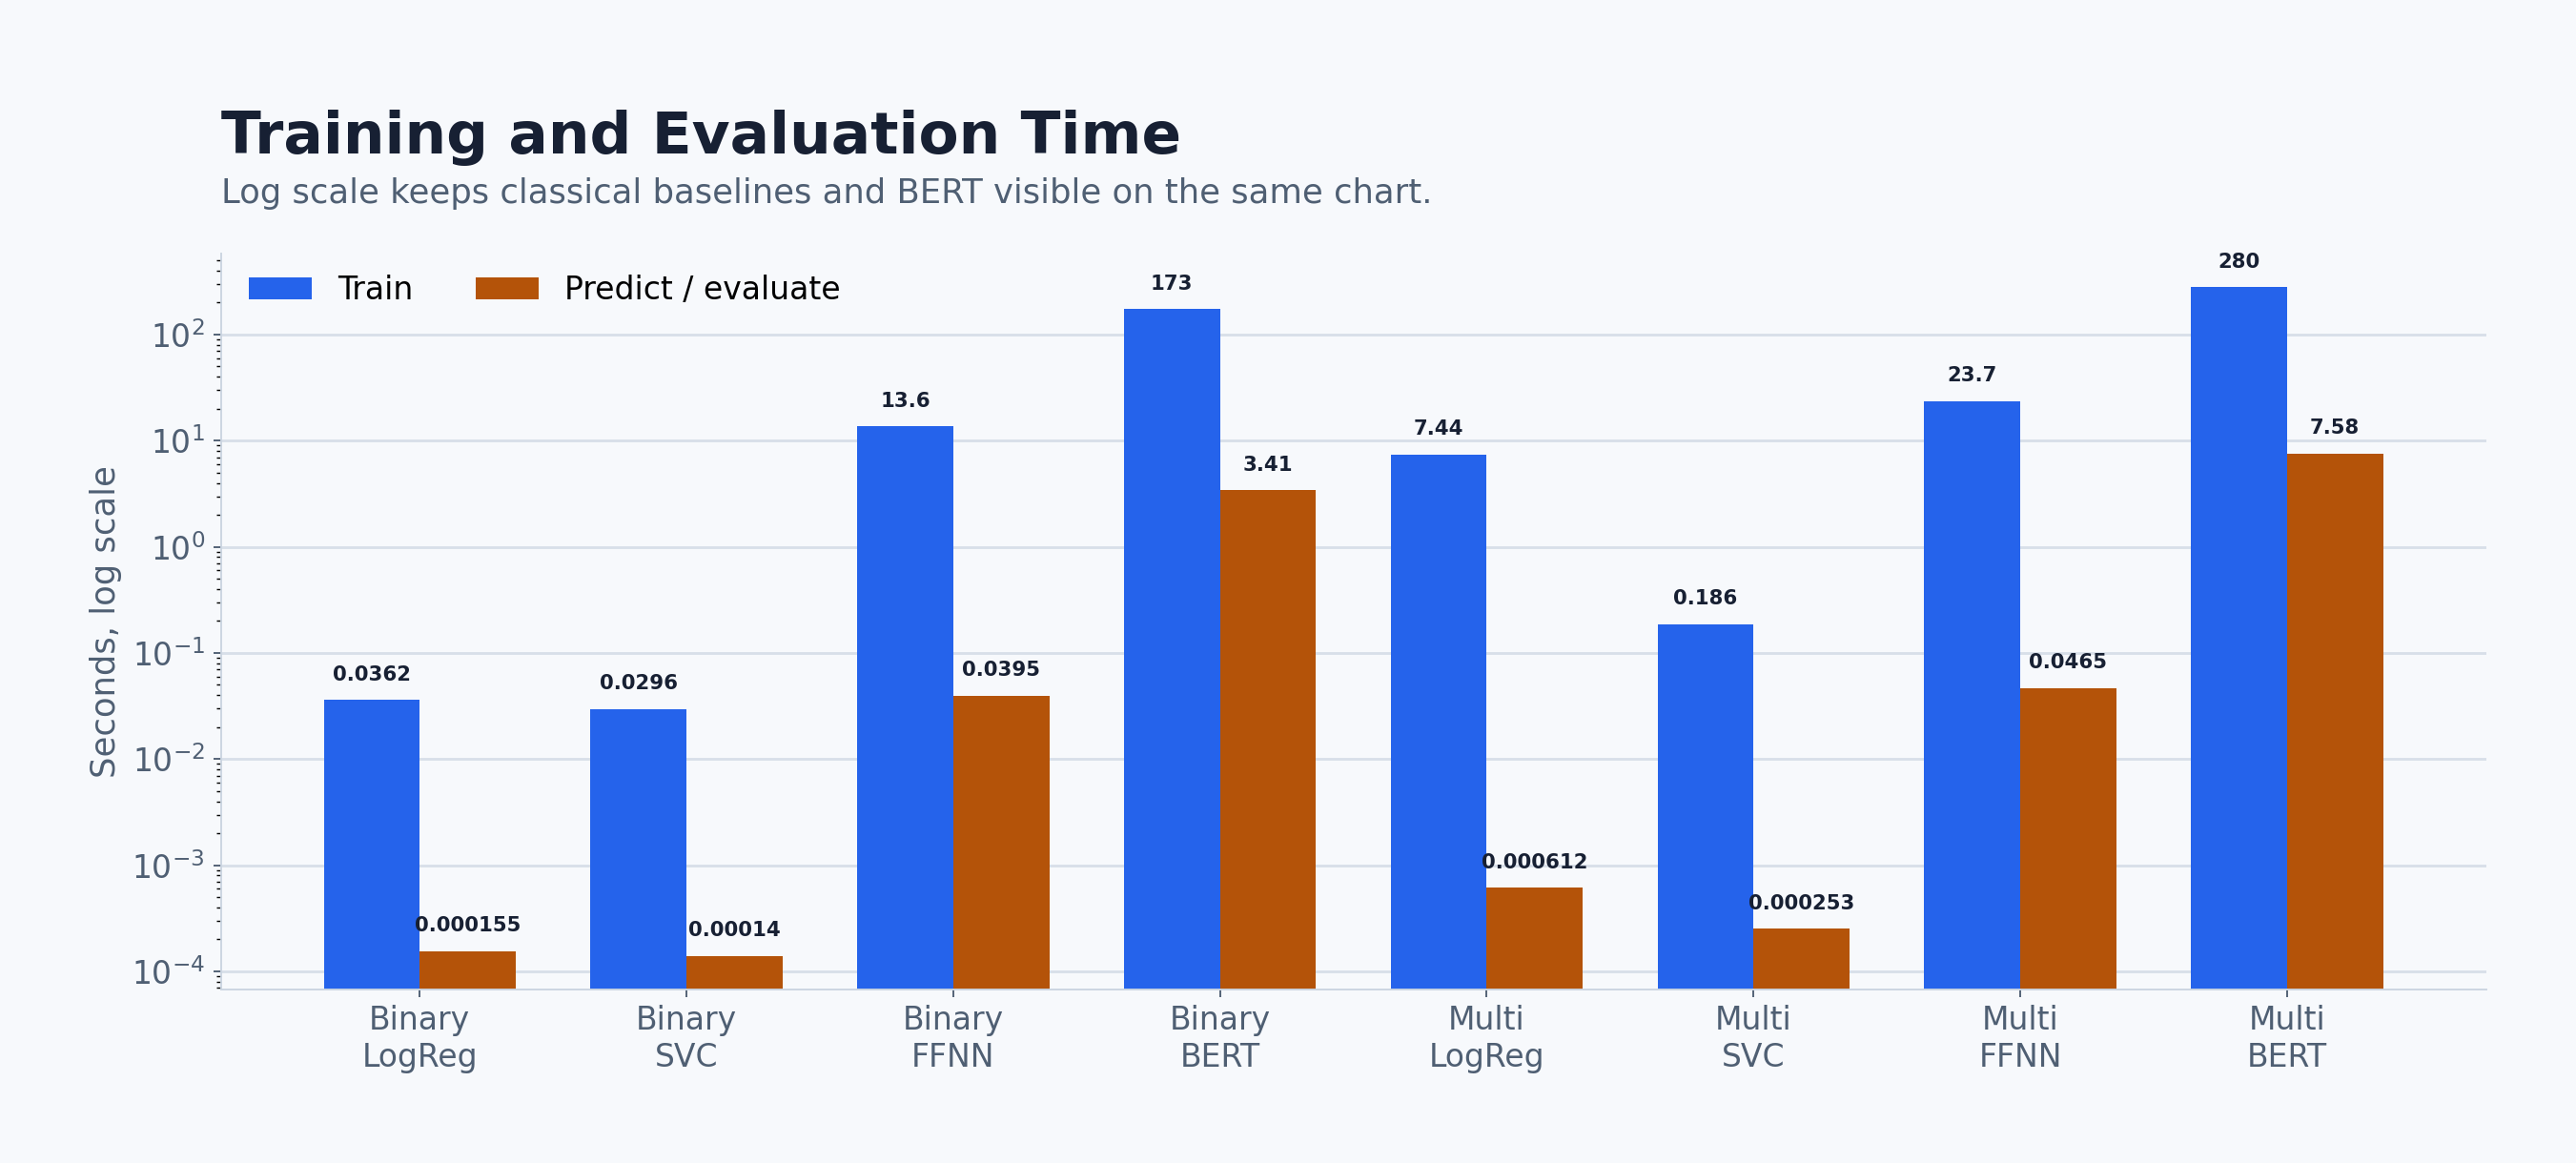
\includegraphics[width=\linewidth]{compute_time_comparison.png}
\caption{Training and evaluation time on a log scale. BERT is the highest-quality model and the only model with substantial compute cost.}
\label{fig:compute}
\end{figure}

\section{Discussion}

The final results support four conclusions. First, label quality changed the project endpoint. Iteration 1 was a useful full-stack weak-label experiment, but the final scientific claim must be based on human-labeled data. Second, strong classical baselines are essential. Logistic Regression and Linear SVC are fast, interpretable, and competitive on binary detection because many positive examples contain overt lexical cues. Third, the FFNN does not justify its added complexity in this dataset; it is close to Linear SVC on binary F1 and below Logistic Regression on multiclass macro F1. Fourth, BERT is the only model that consistently improves aggregate metrics and class-wise F1, with the largest relative value appearing in the five-class task.

The binary and multiclass results should not be collapsed into one conclusion. Binary classification is better for a lightweight moderation gate or user-warning signal. Multiclass classification is better for analysis, policy, and downstream handling because it distinguishes profanity from trolling, derogation, and hate speech. The lower multiclass macro F1 is not a failure of the experiment; it reveals the actual difficulty of the label space.

\section{Limitations and Ethics}

The final dataset is human-labeled, but it still contains short isolated posts without conversation context. Some examples are ambiguous even to a human reader because intent, target, quotation, sarcasm, and social context may be missing. The split is stratified by label, not grouped by author or source, so the reported numbers may overestimate generalization to entirely new communities or writing styles. The minority classes are small: the test split has only 86 Derogatory and 46 Hate Speech examples, so class-wise metrics should be interpreted with appropriate caution.

Ethically, ragebait and abuse detection systems can create both benefits and harms. They can reduce amplification of manipulative or abusive content, but false positives can suppress legitimate anger, satire, reclaimed language, or marginalized speech. A practical deployment should therefore avoid fully automated punitive decisions. The safer use case is assistive triage, transparency, and user-facing friction, combined with human review for high-impact actions. The project also avoids claiming that a binary abusive/ragebait label is the same as a complete theory of harmful speech.

\section{Conclusion}

This project produced a complete final benchmark for ragebait and abusive-language detection. The final package uses a human-labeled dataset, frozen splits, four model families, validation-based model selection, held-out test evaluation, confusion matrices, timing analysis, and targeted error analysis. The best final binary model is BERT with 0.9222 test F1. The best final multiclass model is also BERT with 0.6405 test macro F1. The strongest remaining challenge is not raw model capacity alone; it is the semantic overlap between Trolling, Derogatory abuse, Profanity, and Hate Speech. Future work should test grouped author/source splits, add richer conversation context, and refine annotation guidance for borderline abuse categories.

\begin{thebibliography}{9}

\bibitem{trawling}
\textit{Trawling for Trolling: A Dataset}. arXiv:2008.00525, 2020.

\bibitem{bert}
Jacob Devlin, Ming-Wei Chang, Kenton Lee, and Kristina Toutanova.
\textit{BERT: Pre-training of Deep Bidirectional Transformers for Language Understanding}.
Proceedings of NAACL-HLT, 2019.

\bibitem{sklearn}
F. Pedregosa et al.
\textit{Scikit-learn: Machine Learning in Python}.
Journal of Machine Learning Research, 12, 2825--2830, 2011.

\bibitem{transformers}
Thomas Wolf et al.
\textit{Transformers: State-of-the-Art Natural Language Processing}.
Proceedings of EMNLP: System Demonstrations, 2020.

\bibitem{pytorch}
Adam Paszke et al.
\textit{PyTorch: An Imperative Style, High-Performance Deep Learning Library}.
Advances in Neural Information Processing Systems, 2019.

\bibitem{kaggle-emotion}
aadyasingh55.
\textit{Twitter Emotion Classification Dataset}.
Kaggle, 2023.

\bibitem{kaggle-misleading}
irakozekelly.
\textit{Misleading Posts Driving Discourse on X}.
Kaggle, 2023.

\bibitem{kaggle-alltweets}
speckledpingu.
\textit{Raw Twitter Timelines w/ No Retweets (AllTweets.csv)}.
Kaggle, 2020.

\end{thebibliography}

\end{document}
